\documentclass[tikz, border=10pt]{standalone}
\usepackage{tikz}
\usetikzlibrary{automata, positioning, arrows.meta, calc, shapes.geometric, decorations.pathmorphing}

% --- FONT CONFIGURATION ---
\usepackage{fontspec}
\setmainfont{Noto Sans}

\begin{document}
	
	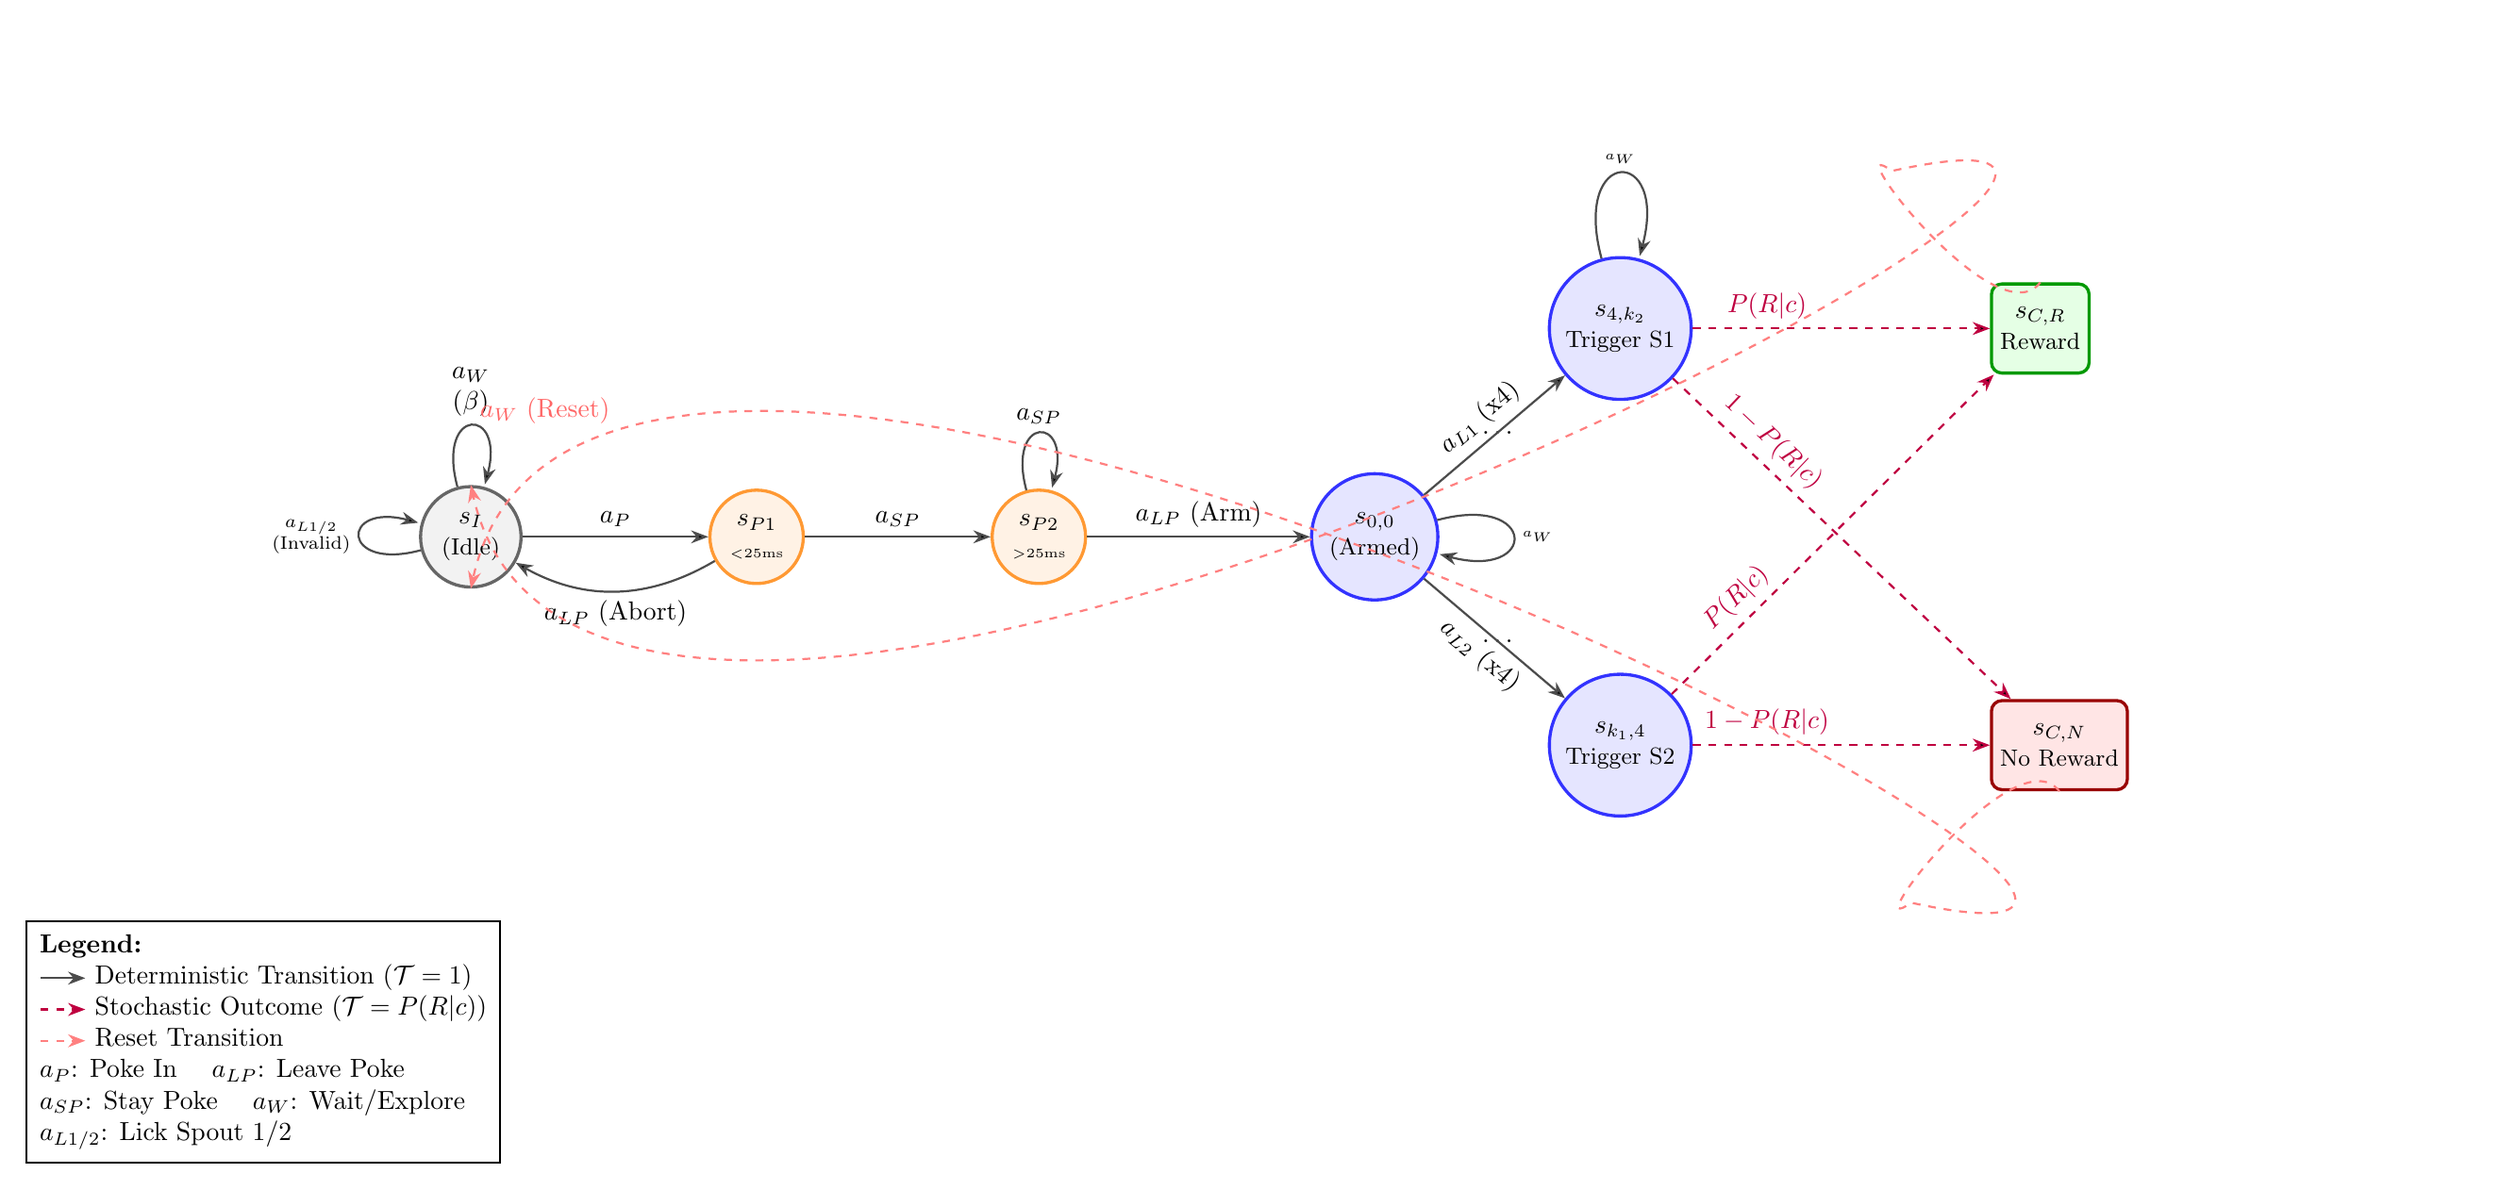
\begin{tikzpicture}[
		>=Stealth, 
		node distance=2.5cm, 
		auto, 
		thick,
		% State Styles
		state_idle/.style={circle, draw=black!60, fill=gray!10, very thick, minimum size=1.2cm, align=center},
		state_poke/.style={circle, draw=orange!80, fill=orange!10, very thick, minimum size=1.2cm, align=center},
		state_armed/.style={circle, draw=blue!80, fill=blue!10, very thick, minimum size=1.4cm, align=center},
		state_outcome/.style={rectangle, rounded corners, draw=green!60!black, fill=green!10, very thick, minimum size=1.2cm, align=center},
		state_fail/.style={rectangle, rounded corners, draw=red!60!black, fill=red!10, very thick, minimum size=1.2cm, align=center},
		% Edge Styles
		action_edge/.style={->, draw=black!70, text=black},
		stochastic_edge/.style={->, draw=purple, dashed, text=purple},
		reset_edge/.style={->, draw=red!50, bend left=45, dashed, text=red!60}
		]
		
		% --- 1. INITIATION PHASE ---
		\node[state_idle] (Idle) {$s_I$\\ \small (Idle)};
		
		\node[state_poke, right=of Idle] (P1) {$s_{P1}$\\ \tiny $<$25ms};
		\node[state_poke, right=of P1] (P2) {$s_{P2}$\\ \tiny $>$25ms};
		
		% --- 2. ACCUMULATION PHASE ---
		\node[state_armed, right=3cm of P2] (Armed) {$s_{0,0}$\\ \small (Armed)};
		
		% Abstract Nodes for Accumulation
		\node[state_armed, above right=1.5cm and 2cm of Armed] (S1_Trig) {$s_{4, k_2}$\\ \small Trigger S1};
		\node[state_armed, below right=1.5cm and 2cm of Armed] (S2_Trig) {$s_{k_1, 4}$\\ \small Trigger S2};
		
		% Ellipsis to imply steps
		\node[draw=none] (dots1) at ($(Armed)!0.5!(S1_Trig)$) {$\dots$};
		\node[draw=none] (dots2) at ($(Armed)!0.5!(S2_Trig)$) {$\dots$};
		
		% --- 3. OUTCOME PHASE ---
		\node[state_outcome, right=4cm of S1_Trig] (CR) {$s_{C,R}$\\ \small Reward};
		\node[state_fail, right=4cm of S2_Trig] (CN) {$s_{C,N}$\\ \small No Reward};
		
		% ================= TRANSITIONS =================
		
		% --- Idle Transitions ---
		\path[action_edge] (Idle) edge node[above] {$a_P$} (P1);
		\path[action_edge] (Idle) edge [loop above] node[align=center] {$a_W$\\($\beta$)} (Idle);
		% NEW: Invalid Lick Loop (Impulsive Behavior)
		\path[action_edge] (Idle) edge [loop left] node[align=center, font=\scriptsize] {$a_{L1/2}$\\(Invalid)} (Idle);
		
		% --- Poke Logic (Nyquist & Abort) ---
		\path[action_edge] (P1) edge node[above] {$a_{SP}$} (P2);
		\path[action_edge] (P2) edge [loop above] node {$a_{SP}$} (P2);
		
		% Abort (Too Short)
		\path[action_edge] (P1) edge [bend left] node[below] {$a_{LP}$ (Abort)} (Idle);
		
		% Success (Arming)
		\path[action_edge] (P2) edge node[above] {$a_{LP}$ (Arm)} (Armed);
		
		% --- Accumulation Logic ---
		% Path to S1 Trigger
		\path[action_edge] (Armed) edge node[sloped, above] {$a_{L1}$ (x4)} (S1_Trig);
		% Path to S2 Trigger
		\path[action_edge] (Armed) edge node[sloped, below] {$a_{L2}$ (x4)} (S2_Trig);
		
		% Wait Tolerance loops
		\path[action_edge] (Armed) edge [loop right] node {\tiny $a_W$} (Armed);
		\path[action_edge] (S1_Trig) edge [loop above] node {\tiny $a_W$} (S1_Trig);
		
		% --- Stochastic Triggers ---
		% Adjusted 'pos' to 0.25 to place labels near start, preventing overlap at the cross
		
		% From S1
		\path[stochastic_edge] (S1_Trig) edge node[above, pos=0.25] {$P(R|c)$} (CR);
		\path[stochastic_edge] (S1_Trig) edge node[above, sloped, pos=0.25] {$1-P(R|c)$} (CN);
		
		% From S2
		\path[stochastic_edge] (S2_Trig) edge node[above, sloped, pos=0.25] {$P(R|c)$} (CR);
		\path[stochastic_edge] (S2_Trig) edge node[above, pos=0.25] {$1-P(R|c)$} (CN);
		
		% --- Resets ---
		% From Consumption back to Idle (Smoother curves)
		
		% Upper Loop (Reward Reset)
		\draw[reset_edge] (CR.north) to[out=90,in=0] ($(CR.north)+(-2,1.5)$) to[out=180,in=90] (Idle.north);
		\node[red!60] at ($(Idle.north)+(1,1)$) {$a_W$ (Reset)};
		
		% Lower Loop (No Reward Reset)
		\draw[reset_edge] (CN.south) to[out=270,in=0] ($(CN.south)+(-2,-1.5)$) to[out=180,in=270] (Idle.south);
		
		
		% ================= LEGEND =================
		% Using inline TikZ drawing instead of math symbols to avoid compilation errors
		\node[draw=black, fill=white, inner sep=5pt, align=left] at (current bounding box.south west) {
			\textbf{Legend:}\\
			\tikz[baseline=-0.5ex]\draw[->, draw=black!70, thick] (0,0) -- (0.6,0); Deterministic Transition ($\mathcal{T}=1$)\\
			\tikz[baseline=-0.5ex]\draw[->, draw=purple, dashed, thick] (0,0) -- (0.6,0); Stochastic Outcome ($\mathcal{T} = P(R|c)$)\\
			\tikz[baseline=-0.5ex]\draw[->, draw=red!50, dashed, thick] (0,0) -- (0.6,0); Reset Transition\\
			$a_P$: Poke In \quad $a_{LP}$: Leave Poke\\
			$a_{SP}$: Stay Poke \quad $a_W$: Wait/Explore\\
			$a_{L1/2}$: Lick Spout 1/2
		};
		
	\end{tikzpicture}
\end{document}